% !TeX root = ../main.tex
% =====================================================================
% Experiments section — v2.1 (review-comment revision).
% Descriptions are purpose/structure only — NO result interpretation;
% \TODO{Results and analysis.} marks every spot where analysis text goes.
% v2.2 (2026-08-17): ablation + transfer results transferred from
% experiments/todo.md (full precision in results-ablations/*.tsv):
%   * tab:main / tab:main-gt: "SOAP (w/o rescoring)" rows moved into
%     tab:weights, which widens to five subsets and gains a base-score row.
%   * tab:scorefn: +L1/L2 rows, random kept, no uncertainty row, FIXED
%     orientations; tab:position: temporal bias split into z-scored/raw;
%     tab:attnsel: w widens to {1,2,3,4,5,all}; fig:transfer: 5x5 -> 4x4
%     (CE dropped), one grid per backbone; tab:synth: shrinks to
%     WW-AG/WW-HC, generators Qwen3.5-9B + GPT-4o, real row refreshed.
%   * Analysis text filled where results exist; figure PDFs still pending
%     (placeholders updated to the new designs).
% v2.3 (2026-08-18): tab:position merged INTO tab:weights (one bracketed
% weight-design table over all five subsets; CE position rows computed for the
% merge — results-ablations/a3_position.tsv now covers CE too). fig:gamma /
% fig:layers / fig:datasize replaced by data tables tab:gamma / tab:layers /
% tab:datasize (marked \note{make this a figure later}); fig:bands and its
% paragraph commented out (covered by tab:scorefn).
% v2.5 (2026-08-31): analysis pass (REDE prose style, artifacts/rede.pdf; data
% from experiments/todo.md + results-ablations/). Every \TODO{Results and
% analysis.} filled: tab:main / tab:main-gt / fig:transfer(b) written fresh;
% the commented drafts for fig:scale, fig:transfer(a), tab:scorefn,
% tab:weights, fig:sensitivity activated. Setup: baseline families matched to
% the table groups (AgenTracer/GraphTracer dropped -- no runs), StepFinder
% described (B1), with-GT adaptation stated (main/data.py: [question, answer]
% context), judge fixed to GPT-4o, empty ablation refs pointed at the Analysis
% section. "Different metrics." stub retired. Old text kept in comments.
% v2.4 (2026-08-24): ablations presented REDE-style (artifacts/rede.pdf).
% tab:gamma / tab:layers -> fig:sensitivity (2x3 strip); tab:attnsel -> appendix;
% tab:transfer + tab:datasize -> fig:transfer (heatmap + lines); tab:scorefn /
% tab:weights restyled (bold best, shaded ours row, row groups). Retired tables
% kept in comments. Figures: scripts/ablations/plot_figures.py ->
% artifacts/ablations/ -> assets/. Mirrors (DeepSeek, TE, val-selected
% transfer) in sections/appendix_ablations.tex (app:deepseek-ablations).
%
% Conventions:
%   * Headline metric: Step-Level Accuracy on the test split, mean +- std
%     over THREE seeds for every dataset (10-seed runs are internal
%     stability checks only, not reported).
%   * Method categories everywhere: Prompt-based methods / Trained LLM
%     attributors / Representation-based methods (StepFinder, OAT, \soap
%     w/o rescoring, \soap full).
%   * Judge/backbone policy (revised 2026-08-03): prompt-based methods
%     run on a CLOSED-SOURCE judge (placeholder \TODO strand in both main
%     tables, name pending); all other methods run on the two open
%     backbones.
%   * GT policy: tab:main is strictly WITHOUT-GT — no method sees the
%     gold answer. tab:main-gt is the with-GT setting: closed-source
%     prompt strand ("Best prompting strategy" = strongest of AAO/SBS/BS,
%     plus CORRECT/CHIEF/RAFFLES) + Qwen3.5-9B strand for the rest
%     (DeepSeek-8B counterpart in app:gt). Per Setup, \soap is ADAPTED to
%     consume the answer there — its w/GT numbers are pending runs.
%     Corpus fact (verified 2026-08-03): every WW/TE JSON carries a
%     non-empty ground_truth (the earlier open-judge reproductions
%     embedded it); all correct-full ground_truth fields are empty. The
%     recorded open-judge prompt numbers therefore fit no cell of the new
%     layout and are preserved in the NOTES comments of both tables, for
%     the appendix.
%   * Resource columns (ex TF/AF, then AD/SL, renamed 2026-08-03):
%     "Actual data" = constructed on actual benchmark trajectories;
%     "Supervised" = construction consumes step-level labels; both empty
%     for pure prompting methods, which have no construction stage.
%     Headers set in \scriptsize to fit.
%   * Ablations: one axis varied, all else fixed to the validation-
%     selected configuration (stated once in the Analysis preamble).
%   * Structure: Setup / Main Results / Analysis (synthetic + ablations).
%
% Macros required in main.tex:
%   \newcommand{\second}[1]{\underline{#1}}   (added 2026-08-03)
%   (\gtmark and \recap are no longer used.)
% Already defined: \PH, \best{}, \cmark, \xmark, \ms{}{}, \TODO{}.
%
% Labels: tab:main, tab:main-gt, fig:scale, fig:transfer, tab:synth,
% tab:scorefn, tab:weights, tab:position, tab:attnsel, fig:gamma,
% fig:layers, fig:bands, fig:datasize.
% (tab:scorers commented out 2026-08-03; base-scorer comparison now lives
% in tab:scorefn.)
% TODO(bib): zhu2026stepfinder is a PLACEHOLDER stub in the .bib — replace
% with the real StepFinder reference. All other keys confirmed present.
% =====================================================================
\section{Experiments}
\label{sec:experiments}
% two tables, w/ wo/ GT. the main table will be absolutely without GT.
% TF, AF -> actual data, actual label.
% remove CORRECT.from the main table.

% remove before in table 3.  don't mix messages.
% Does the effect of backprop rescoring hold across base scorers? -> turn into comparing different base scorers only, not mixing messages. Move to the ablation studies.

% Instead, in the main results add w/ GT in main results. second table.

% putting the synthetic to analysis.
% add attention layer ablation.

% TODO: write method section, revise the main table.

\subsection{Setup}
\label{sec:exp:setup}



\textbf{Datasets.} We evaluate our method \soap on 3 failure-attribution benchmarks comprising 5 subsets:
\textsc{Who\&When}~\citep{whoandwhen}, with algorithm-generated
(\textsc{WW-AG}, 126 trajectories) and hand-crafted
(\textsc{WW-HC}, 58 trajectories) subsets;
\textsc{Correct-Error}~\citep{correct}
(\textsc{CE}, 2{,}226 trajectories);
and \textsc{TraceElephant}~\citep{traceelephant}, with Captain-Agent
(\textsc{TE-Cap}, 85 trajectories) and Magentic-One
(\textsc{TE-Mag}, 91 trajectories) subsets.
They cover trajectories of varying lengths and diverse QA, coding,
and tool-use tasks. Each trajectory is annotated with the decisive-error step
and responsible agent. For each subset, we randomly split trajectories into unlabeled-reference,
validation, and test sets using a $30/20/50\%$ ratio.
The reference annotations are hidden and used only to construct the spectral
matrix $R$; validation labels are used for hyperparameter selection, and test
labels only for final evaluation.
Splitting is performed at the trajectory level.
Full statistics and preprocessing details are provided in
Appendix~\ref{app:datasets}.



% We evaluate on three failure-attribution benchmarks comprising five evaluation subsets, each providing per-trajectory annotations of the decisive-error step and the responsible agent: \text{Who\&When}~\citep{whoandwhen}, with its \emph{algorithm-generated} (\text{WW-AG}, 126 trajectories) and \emph{hand-crafted} (\text{WW-HC}, 58) subsets; \text{CORRECT-Error}~\citep{correct} (\text{CE}, 2{,}226 trajectories); and \text{TraceElephant}~\citep{traceelephant}, with its Captain-Agent (\text{TE-Cap}, 85) and Magentic-One (\text{TE-Mag}, 91) subsets. Together they span short and long trajectories, QA- and code-centric domains, and two generating systems. \hl{Each subset is partitioned \emph{by trajectory} into unlabeled/validation/test splits of $30/20/50\%$.} Full dataset statistics and preprocessing details appear in Appendix~\ref{app:datasets}.


% Following \citet{whoandwhen}, our headline metric is Step-Level Accuracy: the fraction of trajectories whose predicted decisive step exactly matches the annotation. Agent-Level Accuracy, ranking metrics (step@$k$, MRR\textcolor{blue}{give the full name please}), and tolerance variants ($\pm1,\pm2$) are deferred to Appendix~\ref{app:metrics}.

% Rewritten 2026-08-31: families matched to the table row groups (AgenTracer /
% GraphTracer dropped -- never run; StepFinder described per B1,
% experiments/todo.md); the with-GT adaptation of \soap stated here, as the
% tab:main-gt caption promises. Old text:
% \textbf{Baselines.} We compare against three families:
% (i) prompt-based methods, ... (ii) trained LLM attributors, including
% AgenTracer~\citep{agentracer} and GraphTracer~\citep{graphtracer};
% and (iii) representation-based methods, including OAT ... and StepFinder
% \TODO{add description for StepFinder}. ... Since \soap{} never accesses the
% GT answer during inference, we adapt it to compare fairly with baselines in
% the with-GT setting (Table~\ref{tab:main-gt})

% RAFFLES dropped from the comparison 2026-09-06 (kept in related work only).
% Old: "..., the fault-reasoning judge RAFFLES~\citep{raffles}, and the analyzer--verifier ..."
\textbf{Baselines.} We compare \soap against two families of baselines. First, \emph{prompt-based} methods include All-at-Once, Step-by-Step, and Binary Search~\citep{whoandwhen}, the schema-retrieval method CORRECT~\citep{correct}, the causal-graph method CHIEF~\citep{chief}, and the analyzer--verifier diagnoser ErrorProbe~\citep{errorprobe}. These methods ask a judge LLM to name the decisive step. Second, \emph{training-based} methods include OAT~\citep{oat}, which learns successful-trajectory dynamics through one-class training, and StepFinder~\citep{zhu2026stepfinder}, which trains a step classifier on synthetically corrupted trajectories with step-level error labels.
% \textbf{Baselines.} We compare against two families, mirroring the row groups of Table~\ref{tab:main}:
% (i)~\emph{prompt-based} methods, which ask a judge LLM to name the decisive step --- All-at-Once, Step-by-Step, and Binary Search~\citep{whoandwhen}, the schema-retrieval method CORRECT~\citep{correct}, the causal-graph method CHIEF~\citep{chief}, and the fault-reasoning judge RAFFLES~\citep{raffles};
% (ii)~\emph{training-based} methods, which, like \soap, score the trajectory's step representations --- OAT~\citep{oat}, which learns the latent dynamics of successful trajectories through one-class training, and StepFinder~\citep{zhu2026stepfinder}, a step classifier trained on synthetically corrupted trajectories with step-level error labels.


% Our main comparison (Table~\ref{tab:main}) uses the strict \emph{without-ground-truth (GT)} setting, in which no method receives the gold task answer~\citep{whoandwhen}. For the \emph{with-GT} setting we adapt \soap, which never otherwise consults the answer: the gold answer is appended to the task description in the proxy's context, and nothing else changes (Table~\ref{tab:main-gt})


\textbf{Implementation details.} We use Qwen3.5-9B~\citep{qwen3} and DeepSeek-R1-Distill-Llama-8B~\citep{deepseekr1} (DeepSeek-8B) as backbones $\proxy$. We obtain step representations by mean-pooling token hidden states. We select the representation layer, the spectral band $\mathcal{C}$, the attention layer band, and the propagation strength $\gamma$ on the validation set.
% (we show the stability of \soap to each hyperparameter in Section~\ref{sec:exp:analysis})
All training-based baselines use the same two backbones and test data as \soap, with the hyperparameters recommended in their papers. Following~\citet{oat}, we additionally compare with prompt-based baselines with GPT-4o as the judge (results with GPT-5 are in Appendix~\ref{app:prompting-gpt5}). Following \citet{whoandwhen}, we report \emph{Step-Level Accuracy} (additional metrics, including \textit{Agent-level Accuracy} and \textit{top-$k$ Accuracy} are in Appendix~\ref{app:metrics} and~\ref{app:ranked}). Further implementation details are provided in Appendices~\ref{app:implementation} and~\ref{app:baselines}.

% \textcolor{red}{we need to specifically say GPT-4o is used and then put GPT-5 exps in the appendix and refer here.}
% \textbf{Implementation details.}
% We instantiate \soap{} with Qwen3.5-9B~\citep{qwen3} and
% DeepSeek-R1-Distill-Llama-8B~\citep{deepseekr1}.
% % Empty ablation refs pointed at sec:exp:analysis, judge fixed to GPT-4o and
% % the AgenTracer/GraphTracer reimplementation note retired (baselines dropped)
% % 2026-08-31. Old:
% % ... (Ablations are in Appendix~\ref{}) ... (Ablations are in ~\ref{}).
% % We use GPT-\textcolor{blue}{TODO} for the prompt-based methods.
% % \textcolor{blue}{Since neither code nor training data is publicly released
% % for AgenTracer and GraphTracer, we reimplement both following the
% % descriptions in their papers.}
% Step representations are obtained by mean-pooling token hidden states.
% We select the representation layer, the spectral band $\mathcal{C}$, the attention layer band, and the propagation strength $\gamma$ on the
% validation set; \S\ref{sec:exp:analysis} analyzes the sensitivity to each choice.
% The prompt-based methods use GPT-4o as the judge (GPT-5 in Appendix~\ref{app:prompting-gpt5}), evaluated on the same test splits as \soap.
% To ensure a fair comparison, the training-based baselines run on the same two backbones as \soap{} and are evaluated on identical test data, employing the default experimental configurations as outlined in their respective papers.
% Further implementation details appear in Appendices~\ref{app:implementation} and~\ref{app:baselines}.
% \textbf{Metrics.} Following \citet{whoandwhen}, our primary metric is
% \emph{Step-Level Accuracy}, the fraction of trajectories for which the
% predicted decisive step exactly matches the annotation.
% We additionally report Agent-Level Accuracy, Step@$k$, Mean Reciprocal Rank
% (MRR), and $\pm1/\pm2$ tolerance accuracy in
% Appendix~\ref{app:metrics}. \note{add appendix for agent-level and other metrics}

% \textbf{Implementation details.}
% We instantiate \soap{} with Qwen3.5-9B~\citep{qwen3} and
% DeepSeek-R1-Distill-Llama-8B~\citep{deepseekr1}.
% Step representations are obtained by mean-pooling token hidden states (Ablations are in Appendix~\ref{}). We select the representation layer and spectral band $\mathcal{C}$ for spectral decomposition, layer for attention calculation, and propagation strength $\gamma$ on the
% validation set (Ablations are in ~\ref{}). We use GPT-\textcolor{blue}{TODO} for the prompt-based methods. 
% \textcolor{blue}{Since neither code nor training data is publicly released for AgenTracer and
% GraphTracer, we reimplement both following the descriptions in their papers.}
% To ensure a fair comparison, we assess all the other baselines on identical
% test data and backbones, employing the default experimental configurations as outlined in their respective papers.
% Further implementation details appear in Appendices~\ref{app:implementation} and~\ref{app:baselines}. 




% We compare against three families:
% (i)~\emph{prompt-based methods} --- All-at-Once, Step-by-Step, Binary Search~\citep{whoandwhen}, the schema-retrieval method CORRECT~\citep{correct}, the fault-reasoning judge RAFFLES~\citep{raffles}, and the causal-graph method CHIEF~\citep{chief};
% (ii)~\emph{trained LLM attributors} --- AgenTracer~\citep{agentracer} and GraphTracer~\citep{graphtracer}, attributors fine-tuned with reinforcement learning, both reproduced;
% (iii)~a \emph{representation-based method} --- OAT~\citep{oat}, a one-class tracer trained on successful trajectories, the same family as \soap.
% Some baselines can additionally be given the ground-truth task answer. Our main comparison (Table~\ref{tab:main}) is conducted strictly \emph{without} the answer; the with-answer setting is reported separately in Table~\ref{tab:main-gt}. \soap never consults the task answer. CORRECT additionally consumes the gold error annotations of other trajectories through its retrieval protocol (footnoted in Table~\ref{tab:main-gt}). \TODO{Update compared baselines}
% % NOTE: ECHO dropped from the comparison 2026-08-03 (never reproduced); restore
% % here and in a table if that changes.


% \textbf{Implementation details.}  We test our method on two LLM architectures, i.e.,  Qwen3.5-9B~\citep{qwen3} and DeepSeek-R1-Distill-Llama-8B~\citep{deepseekr1}, which are popularly adopted public . To ensure a fair comparison, all baselines are reproduced under the same two backbones rather than transcribed from their original papers. \textcolor{blue}{can we mention a few details here? otherwise there is no detail here really.} The SVD reference $R$ is fit on the train split. All results are reported as mean $\pm$ std over three random seeds, each seed drawing an independent train/validation/test partition.



% NOTE: 10-seed runs on WW/TE are internal stability checks only.
% TODO: fix exact model IDs once final.
\begin{table}[t]
\centering
\footnotesize
\setlength{\tabcolsep}{8pt}
\renewcommand{\arraystretch}{1.04}
\caption{\small \textbf{Main comparison in the \emph{without-ground-truth} setting.} Results are step-level attribution accuracy (\%), averaged over three seeds (std in Appendix~\ref{app:metrics}). No method receives the gold task answer during inference. \textbf{Supervised} marks methods that consume step-level error annotations. Best per column within each block in {bold}, second best \second{underlined}. } 
\vspace{-0.3cm}
\label{tab:main}
\resizebox{\textwidth}{!}{%
\begin{tabular}{@{}lc ccccc@{}}
\toprule
Method & Supervised & \textsc{WW-AG} & \textsc{WW-HC} & \textsc{CE} & \textsc{TE-Cap} & \textsc{TE-Mag} \\
\midrule
\rowcolor{Gray}
\multicolumn{7}{c}{\textit{\textbf{GPT-4o}}}\\
\multicolumn{7}{@{}l}{\textit{Prompt-based methods}}\\
\quad All-at-Once~\citep{whoandwhen}   & \xmark & 14.81 & 6.90 & 28.39 & \second{16.28} & 5.80 \\
\quad Step-by-Step~\citep{whoandwhen}  & \xmark & 20.63 & 13.79 & \second{44.47} & 13.95 & 13.04 \\
\quad Binary Search~\citep{whoandwhen} & \xmark & 22.22 & 4.60 & 9.70 & 9.30 & 6.52 \\
\quad CORRECT~\citep{correct}          & \cmark & 15.34 & 4.60 & 35.12 & 10.85 & \second{13.77} \\
\quad CHIEF~\citep{chief}              & \xmark & \second{25.93} & \second{14.94} & 38.56 & 13.95 & 8.70 \\
% RAFFLES dropped from the comparison 2026-09-06 (kept in related work only).
% \quad RAFFLES~\citep{raffles}          &  & 35.98 & 18.39 & 53.05 & 23.26 & 23.91 \\
% ErrorProbe GPT-4o row filled 2026-09-07: the paper-mode run landed in
% ../attrib-prompting/outputs-nogt/*/*/gpt-4o/errorprobe_paper/ (full budget; no
% weak variant, no truncated/backward GPT-4o runs); scored on the frozen splits by
% scripts/prompting/evaluate.py -> results-prompting/by_column.tsv, zero missing
% or null predictions. It is best on all five columns of this block, so the block
% now carries full markers (seconds: CHIEF WW-AG/WW-HC, Step-by-Step CE,
% All-at-Once TE-Cap, CORRECT TE-Mag), computed against the printed rows — the
% kept pre-reconciliation numbers, see the RAFFLES discrepancy note in
% documents/main.md. With-GT GPT-4o paper-mode cells (WW-AG 34.92, WW-HC 28.74,
% TE-Cap 30.23, TE-Mag 26.81, no CE) await app:gt.
\quad ErrorProbe~\citep{errorprobe}    & \xmark & \textcolor{gray}{\best{38.62}} & \textcolor{gray}{\best{21.84}} & \textcolor{gray}{\best{59.52}} & \textcolor{gray}{\best{27.13}} & \textcolor{gray}{\best{28.26}} \\
\midrule
\rowcolor{Gray}
\multicolumn{7}{c}{\textit{\textbf{Qwen3.5-9B}}}\\
\multicolumn{7}{@{}l}{\textit{Prompt-based methods}}\\
% Open-judge prompt rows filled 2026-09-03: the backbone itself is the judge,
% scored on the frozen seed-split test sets (tables/open_backbones_step_without_gt.tsv;
% scripts/tables/open_backbone_rows.py <- results-prompting/by_column.tsv; see
% experiments/todo.md B2). Best/second markers recomputed per block: RAFFLES
% takes CE and TE-Mag in this block (73.14 / 23.91 vs SOAP 61.78 / 23.19).
\quad All-at-Once~\citep{whoandwhen}    &    \xmark    & 17.46 & 11.49 & 33.47 & 4.65 & 1.45 \\
\quad Step-by-Step~\citep{whoandwhen}   &    \xmark    & 10.58 & 16.09 & 31.15 & 14.73 & 10.87 \\
\quad Binary Search~\citep{whoandwhen}  &    \xmark    & 2.65 & 13.79 & \second{59.92} & 0.78 & 5.07 \\
\quad CORRECT~\citep{correct}       & \cmark & 29.10 & 3.45 & 36.35 & 7.75 & 2.90 \\
\quad CHIEF~\citep{chief}         &     \xmark   & 28.57 & 3.45 & 29.39 & 3.88 & 2.17 \\
% RAFFLES dropped from the comparison 2026-09-06 (kept in related work only). Markers recomputed: \soap best everywhere,
% ErrorProbe second except CE (Binary Search 59.92).
% \quad RAFFLES~\citep{raffles}       &        & \second{46.03} & \second{27.59} & \best{73.14} & \second{29.46} & \second{23.91} \\
% ErrorProbe row switched to the paper mode 2026-09-06 (`errorprobe_paper`: MAST
% tags -> backward trace -> Strategist/Investigator/Arbiter; same scoring path,
% tables/open_backbones_step_without_gt.tsv). The earlier modes, for reference:
% truncated-history (the row until now): 20.63 / 18.39 / 53.40 / 21.71 / 21.74;
% backward-tracing (never run on CE): 5.82 / 11.49 / -- / 3.10 / 7.25.
% 2026-09-06 (user request): the row now comes from the `qwen3.5-9b-weak` judge --
% the SAME Qwen3.5-9B checkpoint decoded on a handicapped budget (512 new tokens,
% temperature 1.0, top-p 0.95, 16k window clipped from the front; see
% ../attrib-prompting/baselines/errorprobe/configs/ww.yaml). Paper mode, scored on
% the same frozen splits (tables/open_backbones_step_without_gt.tsv, "Qwen3.5-9B
% (weak)" rows). The full-budget Qwen3.5-9B paper-mode row it replaces:
% 42.33 / 12.64 / 62.42 / 29.46 / 25.36. Weak truncated / backward modes:
% 19.58 / 24.14 / 49.24 / 21.71 / 17.39 and 9.52 / 14.94 / -- / 3.10 / 10.14.
% Markers: \soap is back to second on CE and TE-Mag; RAFFLES alone second on TE-Cap.
\quad ErrorProbe~\citep{errorprobe}    &    \xmark    & \second{39.68} & \second{21.84} & 55.03 & \second{23.26} & \second{20.29} \\
\addlinespace[1pt]
\multicolumn{7}{@{}l}{\textit{Training-based methods}}\\
\quad StepFinder~\citep{zhu2026stepfinder} & \cmark & 15.87 & 13.33 & 30.03 & 18.29 & 6.67 \\
\quad OAT~\citep{oat}                  & \xmark & 16.72 & 10.11 & 56.50 & 15.35 & 18.84 \\
\addlinespace[1pt]\cmidrule(lr){1-7}
\textbf{\soap (ours)}            & \xmark & \best{47.62} & \best{34.48} & \best{61.78} & \best{35.66} & \best{23.19} \\
\midrule
\rowcolor{Gray}
\multicolumn{7}{c}{\textit{\textbf{DeepSeek-R1-Distill-Llama-8B}}}\\
\multicolumn{7}{@{}l}{\textit{Prompt-based methods}}\\
% Open-judge prompt rows filled 2026-09-03, same source as the Qwen block above.
\quad All-at-Once~\citep{whoandwhen}   &    \xmark    & 7.41 & 5.75 & 21.95 & 4.65 & 2.90 \\
\quad Step-by-Step~\citep{whoandwhen}  &    \xmark    & 16.93 & 9.20 & 9.04 & 11.63 & 4.35 \\
\quad Binary Search~\citep{whoandwhen} &   \xmark     & 7.94 & 12.64 & 34.15 & 10.08 & \second{13.77} \\
\quad CORRECT~\citep{correct}       & \cmark & 20.11 & 11.49 & 32.82 & 3.88 & 0.72 \\
\quad CHIEF~\citep{chief}         &     \xmark   & 17.46 & 2.30 & 8.40 & 7.75 & 9.42 \\
% RAFFLES dropped from the comparison 2026-09-06 (kept in related work only). Markers recomputed: ErrorProbe second on WW-AG,
% OAT second on TE-Cap (17.98 vs ErrorProbe 17.05).
% \quad RAFFLES~\citep{raffles}       &        & \second{28.04} & 8.05 & 35.84 & \second{20.16} & 10.87 \\
% ErrorProbe row switched to the paper mode 2026-09-06 (same source as the Qwen
% block). The earlier modes: truncated-history (the row until now, held second
% on TE-Mag): 14.29 / 6.90 / 36.25 / 13.18 / 17.39; backward-tracing (never run
% on CE): 1.06 / 13.79 / -- / 0.00 / 3.62. With the paper mode at 8.70 on
% TE-Mag, second there returns to Binary Search (13.77).
\quad ErrorProbe~\citep{errorprobe}    &    \xmark    & \second{24.34} & 10.34 & 35.97 & 17.05 & 8.70 \\
\addlinespace[1pt]
\multicolumn{7}{@{}l}{\textit{Training-based methods}}\\
\quad StepFinder~\citep{zhu2026stepfinder} & \cmark & 18.94 & 10.80 & 36.91 & 14.73 & 4.20 \\
\quad OAT~\citep{oat}                  & \xmark & 12.70 & \second{15.86} & \second{52.50} & \second{17.98} & 13.04 \\
\addlinespace[1pt]\cmidrule(lr){1-7}
\textbf{\soap (ours)}            & \xmark & \best{45.50} & \best{28.74} & \best{64.68} & \best{42.64} & \best{30.43} \\
\bottomrule
\end{tabular}}
\vspace{-2em}
\end{table}


\subsection{Main Results}
\label{sec:exp:main}
\begin{figure}[t]
\centering
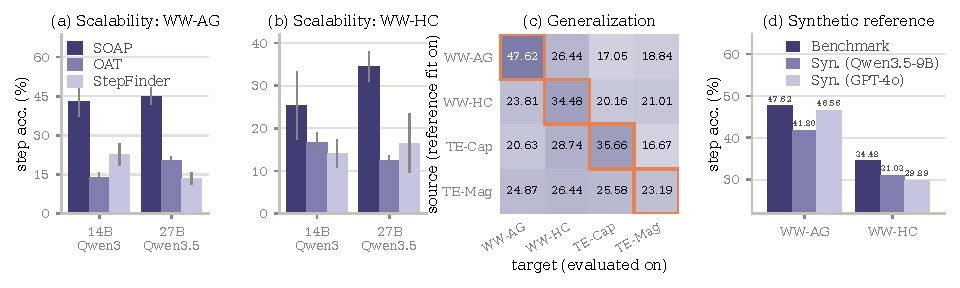
\includegraphics[width=\textwidth]{assets/fig_scale_transfer.pdf}
\vspace{-0.7cm}
\caption{\small (a--b) \textbf{Scalability to larger backbones}, which show the step-level accuracy (\%) on \textsc{WW-AG} and \textsc{WW-HC} using Qwen3-14B and Qwen3.5-27B; error bars denote standard deviations.
{(c)} \textbf{Cross-distribution generalization}, with source datasets as rows and target datasets as columns; outlined diagonal entries correspond to the in-distribution results in Table~\ref{tab:main}.
{(d)} \textbf{Results with synthetic trajectories} generated by Qwen3.5-9B and GPT-4o.
Panels (c) and (d) use Qwen3.5-9B as LLM $\proxy$ for embedding extraction and rescoring. }

% \caption{\textbf{(a) Scalability to larger backbones} on WW-AG. \textbf{(b) Scalability to larger backbones} on WW-HC. Step-level accuracy (\%) with Qwen3-14B and Qwen3.5-27B as the backbone; error bars denote std. \textbf{(c) Generalization across data distributions:} source rows, target columns; the outlined diagonal is the in-distribution result of Table~\ref{tab:main}. \textbf{(d) Results with synthetic trajectories:} the reference is constructed on generated trajectories instead of the real train split. (c) and (d) use backbone Qwen3.5-9B.}
\label{fig:scale}
\label{fig:transfer}
\vspace{-0.7cm}
\end{figure}

\begin{wraptable}{r}{0.45\textwidth}
\vspace{-0.3\baselineskip}
\centering
\scriptsize
\setlength{\tabcolsep}{5.5pt}
\renewcommand{\arraystretch}{0.98}
\caption{\small \textbf{Comparison in the \emph{with-ground-truth} setting.} Results are step-level accuracy (\%) on \textsc{Who\&When}, with the gold task answer provided. All methods use Qwen3.5-9B as the backbone. Marks follow Table~\ref{tab:main}. }
\vspace{-0.3cm}
\label{tab:main-gt}
\resizebox{\linewidth}{!}{%
\begin{tabular}{@{}lc cc@{}}
    \toprule
    Method & Sup. & \textsc{WW-AG} & \textsc{WW-HC} \\
    \midrule
    \multicolumn{4}{@{}l}{\textit{Prompt-based methods}}\\
    % Prompt rows filled 2026-09-05 with the Qwen3.5-9B judge, scored on the frozen
    % with-GT seed triples (tables/open_backbones_step_with_gt.tsv; from
    % results-prompting/by_column.tsv via scripts/tables/open_backbone_rows.py --gt).
    % ErrorProbe = paper mode on the `qwen3.5-9b-weak` judge since 2026-09-06 (same
    % checkpoint, handicapped decoding: 512 new tokens, temperature 1.0, top-p 0.95,
    % 16k window; tables/open_backbones_step_with_gt.tsv "Qwen3.5-9B (weak)"). The
    % full-budget paper-mode row it replaces: 43.92 / 16.09; weak truncated
    % 19.05 / 20.69; weak backward 10.05 / 10.34. WW-AG reads RAFFLES best (46.56),
    % \soap second (43.39), ErrorProbe third (40.74), as the prose says.
    \quad All-at-Once   & \xmark& 21.16 & 11.49 \\
    \quad Step-by-Step  & \xmark& 17.46 & 18.39 \\
    \quad Binary Search & \xmark& 2.12 & 13.79 \\
    \quad CORRECT       & \cmark& 32.28 & 4.60 \\
    \quad CHIEF         & \xmark& 30.69 & 4.60 \\
    % RAFFLES dropped from the comparison 2026-09-06 (kept in related work only).
    % \quad RAFFLES       &       & \best{46.56} & \second{28.74} \\
    \quad ErrorProbe    & \xmark& \second{40.74} & \second{19.54} \\
    \addlinespace[1pt]
    \multicolumn{4}{@{}l}{\textit{Training-based methods}}\\
    \quad StepFinder    & \cmark& 18.52 & 12.87 \\
    \quad OAT           & \xmark& 22.12 & 8.05 \\
    \addlinespace[1pt]\cmidrule(lr){1-4}
    \quad \textbf{\soap (ours)} & \xmark& \best{43.39} & \best{34.48} \\
    \bottomrule
\end{tabular}}
\vspace{-1\baselineskip}
\end{wraptable}

\textbf{Comparison with competitive baselines.} Table~\ref{tab:main} compares \soap with prompt-based and training-based baselines across all five subsets, without access to the gold task answer at inference. With both open-weight backbones, \soap achieves the highest step-level accuracy on every subset. For example, on \textsc{WW-AG} with Qwen3.5-9B, \soap attains 47.62\%, compared with 39.68\% for ErrorProbe~\citep{errorprobe}, the strongest prompt-based baseline, and 16.72\% for OAT~\citep{oat}, the strongest training-based baseline. Its advantage over prompt-based methods using closed-source judges also persists with both GPT-4o and GPT-5; the GPT-5 results are  in Appendix~\ref{app:prompting-gpt5}.  These results demonstrate that step-unlabeled failure trajectories provide an effective source of localization signal, outperforming the success-only trajectories used by OAT and the step-level supervision used by StepFinder. Agent-level results  are provided in Appendix~\ref{app:metrics}.






\noindent \textbf{Results for the with-GT setting.} To assess the effectiveness of \soap under the with-GT setting, we provide the gold task answer to all methods and compare them in Table~\ref{tab:main-gt}. When provided with the ground-truth answer, \soap remains the best method on both subsets, ahead of the strongest prompt-based baseline ErrorProbe~\citep{errorprobe} (43.39 vs.\ 40.74 on \textsc{WW-AG} and 34.48 vs.\ 19.54 on \textsc{WW-HC}), while every training-based baseline trails by more than 20 points (e.g., 22.12 for OAT~\citep{oat} on \textsc{WW-AG}). Results on DeepSeek-8B appear in Appendix~\ref{app:gt}. 


\textbf{Scalability to larger backbones.} To assess scalability, we evaluate \soap on two larger backbones, Qwen3-14B and Qwen3.5-27B. As shown in Figure~\ref{fig:scale}(a-b), \soap achieves stable accuracy on both backbones and outperforms the SOTA baselines (e.g., 44.97 vs.\ 22.65 for StepFinder~\citep{zhu2026stepfinder} on \textsc{WW-AG}). These results confirm that \soap remains effective on larger backbones.

\textbf{Generalization across data distributions.} We construct the reference on a source subset and directly evaluate \soap on a different target subset, for every pair among \{\textsc{WW-AG}, \textsc{WW-HC}, \textsc{TE-Cap}, \textsc{TE-Mag}\}. As shown in Figure~\ref{fig:transfer}(c), \soap transfers across subsets: for example, constructing on \textsc{WW-HC} and testing on \textsc{TE-Mag} achieves 21.01, compared with the in-domain result of 23.19. These results indicate that the spectral reference captures failure structure that can be generalizable in practice. Results on DeepSeek-8B appear in Appendix~\ref{app:transfer}.






% Re-wrapped 2026-09-01 (was un-wrapped 2026-08-31 while the section was unfinished).
\textbf{Results with synthetic trajectories.}  
Our main results construct $R$ from existing benchmark trajectories. We further examine whether alternative synthetic trajectories can serve as the reference while retaining Qwen3.5-9B as the attribution backbone. We generate the same number of trajectories using either Qwen3.5-9B itself or GPT-4o as an external generator, while keeping the original validation and test splits unchanged. As shown in Figure~\ref{fig:transfer}(d), both synthetic references remain effective. For example, the GPT-4o-generated reference achieves 46.56 on \textsc{WW-AG}, close to 47.62 using the original training trajectories. Thus, \soap can construct its reference space from synthetic trajectories, 
either when generated by the same or a different model. 
Generation details are provided in Appendix~\ref{app:synth}.




\begin{figure}[t]
\centering
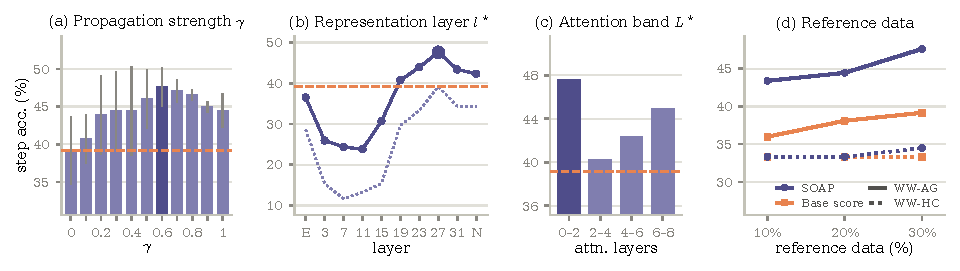
\includegraphics[width=\textwidth]{assets/fig_ablations.pdf}
\vspace{-0.9cm}
\caption{\small \textbf{Ablation studies.} Sensitivity to (a) propagation strength $\gamma$, (b) representation layer $l^\star$, (c) attention layer band $L^\star$, and (d) the amount of unlabeled reference data. All experiments use Qwen3.5-9B. Panels (a--c) vary one hyperparameter at a time from the selected \textsc{WW-AG} configuration used in Table~\ref{tab:main}. Dark bars and enlarged markers denote the selected values; the orange dashed line denotes the base score without rescoring ($\gamma=0$), and the dotted curve in (b) reports the base score at each layer. Panel (d) constructs $R$ using $10\%$, $20\%$, or $30\%$ of the reference corpus and reports results on \textsc{WW-AG} and \textsc{WW-HC}. Best viewed in color. }
\label{fig:datasize}
\vspace{-0.5cm}
\end{figure}


\vspace{-1em}

\subsection{Analysis}
\label{sec:exp:analysis}


\begin{wraptable}{r}{0.40\textwidth}
% \vspace{-0.4\baselineskip}
\centering
\footnotesize
\setlength{\tabcolsep}{4pt}
\renewcommand{\arraystretch}{1.04}
\vspace{-0.3cm}
\caption{\small \textbf{Comparison with alternative scoring functions.} Results are step-level accuracy (\%) on backbone Qwen3.5-9B, with no rescoring.
}
\vspace{-0.3cm}
\label{tab:scorefn}
\resizebox{\linewidth}{!}{%
    \begin{tabular}{l cc}
    \toprule
    Scoring function & \textsc{WW-AG} & \textsc{WW-HC} \\
    \midrule
    Perplexity           & 3.70  & 8.05 \\
    Random subspace      & 13.23 & 9.20 \\
    Top subspace         & 12.70 & \best{33.33} \\
    Tail subspace        & 6.35  & 6.90 \\
    Full spectrum        & 12.17 & 31.03 \\
    Norm $\ell_1$        & 18.52 & 18.39 \\
    Norm $\ell_2$        & 14.29 & 26.44 \\
    \rowcolor{Gray}
    \textbf{Spectral band (ours)} & \best{39.15} & \best{33.33} \\
    \bottomrule
    \end{tabular}}
\vspace{-1.8\baselineskip}
\end{wraptable}
\textbf{Comparison with alternative scoring functions.} We compare the spectral base score (Eq.~\ref{eq:base-score}) with seven alternatives in Table~\ref{tab:scorefn}: step perplexity, projection to random subspace, top subspace, tail subspace, full spectrum, and the $\ell_1$ and $\ell_2$ norms of LLM step embeddings (details in Appendix~\ref{app:implementation}). Our spectral band (Eq.~\ref{eq:spectral-band}) remains the best on both subsets, and the best alternative reaches only 18.52 on \textsc{WW-AG}, compared with 39.15 for ours. These results indicate that the decisive-error signal lies more likely in a selected spectral band  than in LLM predictive likelihood or embedding magnitude.

\textbf{Sensitivity to the hyperparameters.} We vary the propagation strength $\gamma$ (Eq.~\ref{eq:recap}), representation layer $l^\star$ for base score calculation (Eq.~\ref{eq:base-score}), and layer band $L^\star$ for attention mass calculation (Eq.~\ref{eq:dependency-weight}) one at a time. Here, $L^\star$ specifies the group of attention blocks averaged to estimate step dependencies (cf. Appendix~\ref{app:implementation} for details). As shown in Figure~\ref{fig:datasize}, propagation consistently improves over the base score and peaks at $\gamma=0.6$, while later representation layers perform best. The earliest attention band performs best, suggesting that lower attention blocks provide clearer dependency signals, although all bands improve over the base score.  Extended ablations on subsets \textsc{WW-HC}, \textsc{TE-Cap}, \textsc{TE-Mag}, backbone DeepSeek-8B are in Appendix~\ref{app:deepseek-ablations}.

% Reduced to WW-AG / WW-HC / CE and re-set as a wraptable 2026-09-08 (review
% request: match the other ablations). The TE-Cap / TE-Mag columns moved to
% tab:weights-app (app:weights). The full five-column table it replaces:
%   Rescoring design          WW-AG  WW-HC  CE     TE-Cap TE-Mag
%   Base score (no rescoring) 39.15  33.33  61.38  33.33  21.01
%   Uniform, unnormalized     16.93  16.09  57.85  14.73  5.07
%   Uniform, normalized       40.21  34.48  60.78  35.66  15.94
%   Temporal bias, z-scored   40.74  34.48  61.62  34.11  21.01
%   Temporal bias, raw        22.22  3.45   41.65  6.20   5.07
%   Earliest of top-5         21.16  14.94  4.51   9.30   5.07
%   Attention-guided (ours)   47.62  34.48  61.78  35.66  23.19

% Weight rows replace only the dependency weights; position rows replace the whole correction ($\lambda$ selected per column from $\{0.1,\dots,1.0\}$; \emph{z-scored} standardizes the base score within each trajectory before adding the bias, \emph{raw} does not). The last row equals \soap in Table~\ref{tab:main}. Best in \best{bold}. TE-Cap and TE-Mag are in Appendix~\ref{app:weights}.


\begin{wraptable}{r}{0.49\textwidth}
\vspace{-1.1\baselineskip}
\centering
\footnotesize
\setlength{\tabcolsep}{4pt}
\renewcommand{\arraystretch}{1.04}
\caption{\small \textbf{Alternatives to attention-guided rescoring.}
Step-level accuracy using Qwen3.5-9B; all methods share the same base score.}
\label{tab:weights}
\vspace{-0.3cm}
\begin{tabularx}{\linewidth}{l*{2}{>{\centering\arraybackslash}X}}
\toprule
Rescoring design & \textsc{WW-AG} & \textsc{CE} \\
\midrule
Base score (no rescoring) & 39.15 & 61.38 \\
\addlinespace[2pt]
\multicolumn{3}{@{}l}{\textit{Content-agnostic}} \\
\quad Uniform, unnormalized & 16.93 & 57.85 \\
\quad Uniform, normalized   & 40.21 & 60.78 \\
\addlinespace[2pt]
\multicolumn{3}{@{}l}{\textit{Position heuristics}} \\
\quad Temporal bias, std. & 40.74 & 61.62 \\
\quad Temporal bias, base      & 22.22 & 41.65 \\
\quad Earliest of top-$5$      & 21.16 & 4.51 \\
\addlinespace[2pt]
\rowcolor{Gray}
\textbf{Attention-guided (ours)} & \best{47.62} & \best{61.78} \\
\bottomrule
\end{tabularx}
\vspace{-1.3\baselineskip}
\end{wraptable}

\textbf{Importance of attention-guided rescoring.}
% Table~\ref{tab:weights} keeps the spectral base score fixed and replaces attention-guided rescoring with simpler alternatives (details in Appendix~\ref{app:implementation}). \emph{Uniform, normalized} averages all successor scores equally, whereas \emph{uniform, unnormalized} sums them, favoring early steps with more successors. \emph{Temporal bias} favors earlier steps by subtracting a position-dependent penalty $\lambda t/T$, which increases for later steps. The \emph{base} variant subtracts this penalty directly from the base score $\Sbase(s_t)$, whereas the \emph{standardized} variant first standardizes the base scores within each trajectory and then applies the same penalty. \emph{Earliest of top-$5$} selects the earliest among the five highest-scoring steps. Attention-guided rescoring performs best on both subsets, reaching 47.62 on WW-AG compared with 40.74 for the strongest alternative. This shows that the gain arises from selectively weighting downstream evidence through attention, rather than uniform aggregation or positional bias.
Table~\ref{tab:weights} keeps the spectral base score fixed and replaces attention-guided rescoring with simpler alternatives (details in Appendix~\ref{app:implementation}). \emph{Uniform, normalized} averages all successor scores equally, whereas \emph{uniform, unnormalized} sums them, favoring early steps with more successors. \emph{Temporal bias} subtracts a penalty $\lambda t/T$ that grows with the step position $t$, either from the base score $\Sbase(s_t)$ directly (\emph{base}) or after standardizing the base scores within each trajectory (\emph{standardized}). \emph{Earliest of top-$5$} selects the earliest among the five highest-scoring steps. Attention-guided rescoring performs best on both subsets, reaching 47.62 on \textsc{WW-AG} compared with 40.74 for the strongest alternative. This shows that the gain arises from selectively weighting downstream evidence through attention, rather than uniform aggregation or positional bias.
% 2026-09-14: the closing sentence "The same pattern holds on TE-Cap and TE-Mag
% (Appendix~\ref{app:weights})" was removed because the rescoring-design mirror
% (app:weights, tab:weights-app) is commented out in the appendix. The five-column
% numbers it referred to are kept in the comment above tab:weights.



% \begin{wraptable}{r}{0.47\textwidth}
% \vspace{-0.9\baselineskip}
% \centering
% \footnotesize
% \setlength{\tabcolsep}{4pt}
% \renewcommand{\arraystretch}{1.04}
% \caption{\small \textbf{Alternatives to attention-guided rescoring.} Step-level accuracy (\%), Qwen3.5-9B; all rows share the spectral base score. 
% }
% \vspace{-0.3cm}
% \label{tab:weights}
% \resizebox{\linewidth}{!}{%
% \begin{tabular}{l ccc}
% \toprule
% Rescoring design & WW-AG & WW-HC & CE \\
% \midrule
% Base score (no rescoring)& 39.15 & 33.33 & 61.38 \\
% \addlinespace[2pt]
% \multicolumn{4}{@{}l}{\textit{Content-agnostic weights}} \\
% \quad Uniform, unnormalized& 16.93 & 16.09 & 57.85 \\
% \quad Uniform, normalized& 40.21 & \best{34.48} & 60.78 \\
% \addlinespace[2pt]
% \multicolumn{4}{@{}l}{\textit{Position heuristics}} \\
% \quad Temporal bias, z-scored& 40.74 & \best{34.48} & 61.62 \\
% \quad Temporal bias, raw& 22.22 & 3.45  & 41.65 \\
% \quad Earliest of top-$5$& 21.16 & 14.94 & 4.51  \\
% \addlinespace[2pt]
% \rowcolor{Gray}
% Attention-guided (ours)& \best{47.62} & \best{34.48} & \best{61.78} \\
% \bottomrule
% \end{tabular}%
% }
% \vspace{-0.9\baselineskip}
% \end{wraptable}
% \textbf{Importance of attention-guided rescoring.} Table~\ref{tab:weights} keeps the base score and $\gamma$ fixed and replaces the dependency weights of Eq.~\ref{eq:backward-evidence} with simpler rules. \emph{Uniform, normalized} averages the base scores of all later steps with equal weight; \emph{uniform, unnormalized} sums them instead, so early steps collect more terms. \emph{Temporal bias} penalizes later steps by subtracting  $\lambda\,t/T$ from the base score of step t in a trajectory of T steps; its z-scored variant first standardizes the base scores within each trajectory, while the raw variant does not. \emph{Earliest of top-$5$} predicts the earliest of the five highest-scoring steps. Attention-guided weights match or outperform every alternative on all three subsets: on WW-AG they reach 47.62, while the plain average reaches 40.21, the best position heuristic 40.74, and the rules that push blame early collapse (16.93 and 21.16). These results indicate that the gain comes from how much successors are selected by the attention, not from simply averaging over successors or from preferring early steps. The same picture holds on TE-Cap and TE-Mag (Appendix~\ref{app:weights}).





\begin{wrapfigure}{r}{0.40\textwidth}
\vspace{-0.9\baselineskip}
\centering
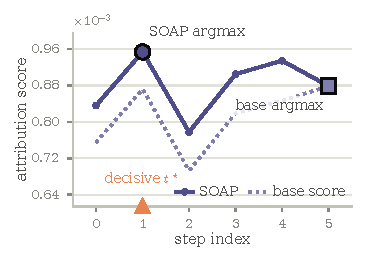
\includegraphics[width=0.95\linewidth]{assets/scores_captain_traj1.pdf}
\vspace{-0.3cm}
\caption{\textbf{Qualitative example.} Per-step scores on a \textsc{TE-Cap} trajectory with backbone Qwen3.5-9B. The base score (dotted) peaks late; \soap (solid) lifts the decisive error $t^\star$ (orange marker) to the top. The large square and circle mark each score's argmax.}
\label{fig:qualitative}
\vspace{-0.9\baselineskip}
\end{wrapfigure}
\textbf{Quantity of unlabeled reference data.} We construct $R$ on random subsamples covering $\{10, 20, 30\}\%$ of the corpus, with the validation and test splits fixed. As shown in Figure~\ref{fig:datasize}(d), \soap needs little reference data: with a third of our 30\% train split (twelve trajectories on \textsc{WW-AG} and six on \textsc{WW-HC}), accuracy is within a few points of the full-data result (43.39 vs.\ 47.62 on \textsc{WW-AG}). These results indicate that a handful of unlabeled trajectories suffices to construct the reference, showcasing the practicality of our approach.



% \textbf{Qualitative example.} Figure~\ref{fig:qualitative} shows a TE-Cap trajectory on which rescoring flips the prediction from wrong to right. The base score peaks late, on an Orchestrator turn that only summarizes earlier steps. The dependency weights route this late contamination back to the decisive error, a malformed program produced by the extraction agent four steps earlier. Further detailed textual trajectories are shown in Appendix~\ref{app:qualitative}.
% \textbf{Qualitative example.} In the TE-Cap trajectory of Figure~\ref{fig:qualitative}, the base score peaks on a late Orchestrator turn only summarizing earlier steps. Rescoring routes that late signal back to the decisive error, a malformed program produced by the code agent four steps earlier, and corrects the prediction. More textual examples are in Appendix~\ref{app:qualitative}.

\textbf{Qualitative example.} In the \textsc{TE-Cap} trajectory of Figure~\ref{fig:qualitative}, the base score peaks on the final Orchestrator turn, which only restates the wrong answer. Rescoring routes that late signal back to the decisive error four steps earlier, where the extraction expert misreads the program's structure and proposes the wrong fix, and corrects the prediction. More textual examples are in Appendix~\ref{app:qualitative}. 




% \textbf{Additional analysis.} Due to space limitations, we defer additional experiments to the Appendix, including (1) efficiency comparison between \soap and other baselines (Appendix [to be added]), and  (2) the selection of context window $w$ in building $\mathcal{P}_t$  the rescoring function (Appendix~\ref{app:window}.

% \textbf{Additional analysis.} Due to space limitations, we defer additional experiments to the Appendix, including (1) the inference cost of \soap and the baselines (Appendix~\ref{app:compute}) and (2) the choice of the window $w$ that bounds the predecessor set $\mathcal{P}_t$ in rescoring (Appendix~\ref{app:window}). \textcolor{red}{add more}
% \textcolor{red}{efficiency comparison to be in the appendix, put the context window thing here, but take a look my wording in the method section to  accurately describe}
% \textbf{Additional analysis.} Due to space limitations, we defer additional experiments to the Appendix, including (1) the cost analysis of \soap and the baselines (Appendix~\ref{app:compute}), (2) the choice of the window that bounds the predecessor set $\mathcal{P}_t$ in rescoring (Appendix~\ref{app:window}), (3) pooling strategies of step representation (Appendix~\ref{app:pooling}), (4) the hyperparameter sensitivity w.r.t backbones and subsets (Appendix~\ref{app:sensitivity}), and (5) the extended results on larger backbones (Appendix~\ref{app:proxies}), synthetic references (Appendix~\ref{app:synth-results}), and the quantity of reference data (Appendix~\ref{app:datasize}).

\textbf{Additional analysis.} Due to space limitations, we defer additional experiments to the Appendix: cost analysis~(\ref{app:compute}), context window $w$ in constructing $\mathcal{P}_t$~(\ref{app:window}), representation pooling~(\ref{app:pooling}), hyperparameter sensitivity~(\ref{app:sensitivity}), trivial baselines~(\ref{app:length}), sensitivity to the reference corpus~(\ref{app:reference-controls}), a supervised probe comparison~(\ref{app:probe}), and extended results on larger backbones~(\ref{app:proxies}), synthetic references~(\ref{app:synth-results}), and reference data quantity~(\ref{app:datasize}).

\vspace{-1em}